\documentclass[12pt,a4paper]{article} 
\usepackage[utf8]{inputenx} 
\usepackage[spanish]{babel} 
\usepackage[left=2cm,right=2cm,top=2cm,bottom=2cm]{geometry}
\usepackage{scrextend}
\usepackage{marvosym}
\usepackage{pifont} % Generación de símbolos especiales
\usepackage{textcomp}
\usepackage{newpxtext}
\usepackage{newpxmath}
\usepackage[T1]{fontenc} % Codificación de salida    
\usepackage{microtype} % Mejoras de microtipografía en la obtención de PDF (sólo para pdflatex)
\usepackage[hyphens]{url} % Para escritura de URL
\urlstyle{sf} % Estilo de URL sin serifas para que tengan un mejor aspecto
\usepackage{tikz}
% Paquetes para obtener un mayor control de las listas
\usepackage{paralist} % Mayor control de listas
\usepackage{multicol} % Elementos en varias columnas
\usepackage[breaklinks]{hyperref}
\usepackage{graphicx}
\usepackage{caption}
\captionsetup[figure]{labelformat=empty}
\author{Julián García Sánchez \and Iván Illán Barraya \and Alejandro Medina Jiménez \and Javier Monescillo Buitrón}
\title{Implementación de un procesador de lenguajes para Autómatas de Moore}
\date{\today}
%%%%%%%%%%%%%%

\begin{document}
	
	\maketitle
	
	\begin{figure}[h]
		\centering
		
\includegraphics[width=0.25
		\linewidth]{img/image004}
		\caption{}
		\label{fig:image004}
	\end{figure}

	\newpage
	\tableofcontents
	\newpage
	
	\section{¿Qué es un autómata de Moore?}
	En Teoría de la computación una \textbf{Máquina de Moore} es un autómata de estados finitos para el cual la salida en un momento dado sólo depende de su estado en ese momento, mientras la transición al siguiente estado depende del estado en que se encuentre y de la entrada introducida.
	El diagrama de estados para una máquina de Moore incluirá una señal de salida para cada estado. \cite{Moore1}
	
	\begin{figure}[h]
		\centering
		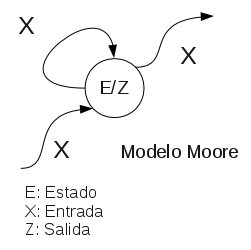
\includegraphics[width=0.5
		\linewidth]{img/Modelo-moore}
		\caption{Ejemplo de Máquina de Moore simple}
		\label{fig:modelo-moore}
	\end{figure}
	
	
	
	El nombre de \textbf{Máquina de Moore} viene de su promotor Edward F. Moore, un pionero de las máquinas de estados, quien escribió \textit{Gedanken-experiments on Sequential Machines,} pp 129-153, Estudios de Autómatas, Anuales de los Estudios Matemáticos, no. 34, Princenton Universityy Press, Princenton, N.J., 1956. \cite{Moore1}
	
	\subsection{Definición formal}
	Una máquina de Moore se define como una 6-tupla:
	\[ Mmor = (S,S_{0},\Sigma,\Lambda,T,G)  \]
	donde definimos los siguientes elementos:
	\begin{itemize}
		\item S: es un conjunto finito de estados.
		\item $S_{0}$: es el estado inicial, y además es un elemento de S.
		\item $\Sigma$: un conjunto finito llamado alfabeto de entrada.
		\item $\Lambda$: un conjunto finito llamado el alfabeto de salida.
		\item $T$ : una función de transición $T: S \times \Sigma \rightarrow S$ mapeando un estado y una entrada al siguiente estado.
		\item $G$ función de salida $G : S \rightarrow \Lambda $ mapeando cada estado al alfabeto de salida.
	\end{itemize}
	\clearpage

	
	\newpage
	\subsection{Ejemplo propuesto}
	Definimos una Máquina de Moore para regular el tráfico en el siguiente cruce con los cuatro semáforos:
		
	\begin{figure}[h]
		\centering
		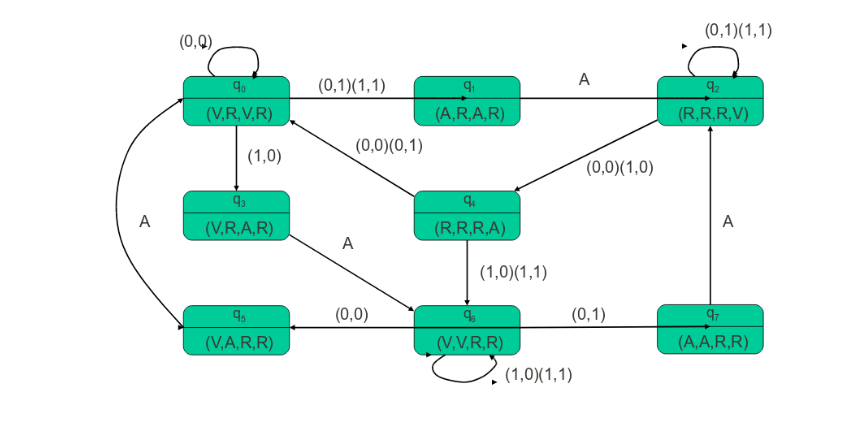
\includegraphics[width=0.4
		\linewidth]{img/4}
		\caption{}
		\label{fig:4}
	\end{figure}

El alfabeto de entrada $\Sigma$: {(0,0),(0,1),(1,0),(1,1)}

	\begin{itemize}
		\item (a,b), donde a es el estado para el sensor $\alpha$ y b para el sensor $\beta$
		\item 0 indica que no hay coches en la cola
		\item 1 indica que hay coches en la cola
	\end{itemize}

El alfabeto de salida $\Lambda$: { ($a_{1},a_{2},a_{3},a_{4}$ donde $a_{i}\epsilon$ (A,V,R) )
	\begin{itemize}
		\item $a_{1}$ es el estado del semáforo 1
		\item $a_{2}$ es el estado del semáforo 2
		\item $a_{3}$ es el estado del semáforo 2
		\item $a_{4}$ es el estado del semáforo 2
	\end{itemize}

	\begin{center}
		\textit{El diagrama de estados sería el siguiente}
	\end{center}

	\begin{figure}[h]
		\centering
		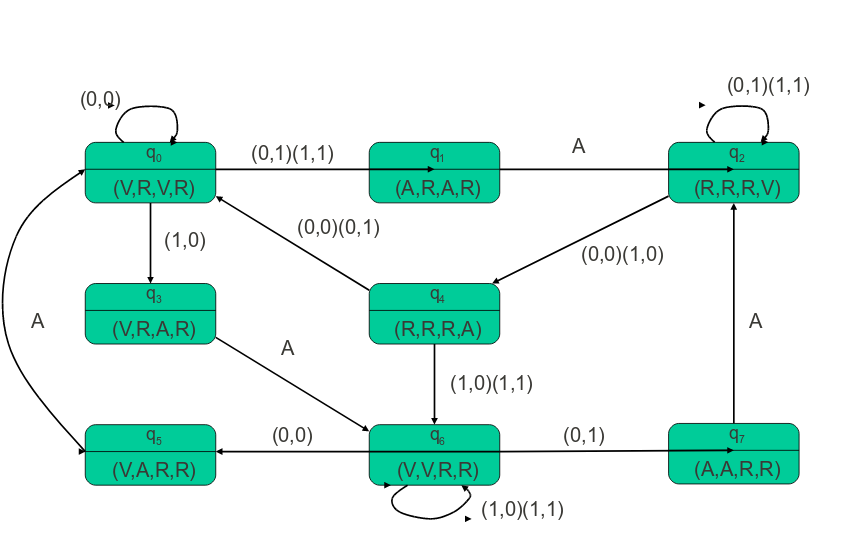
\includegraphics[width=0.7
		\linewidth]{img/3}
		\caption{}
		\label{fig:3}
	\end{figure}

	\newpage
	\section{Presentación del problema}
	La práctica consiste en el diseño de un procesador de lenguajes cuya entrada estará formada por una o varias máquinas de Moore y su salida será código en un lenguaje de alto nivel que lo represente, en nuestro caso Java.
	\newline
	\newline
	Los conocimientos en la materia serán útiles en las distintas etapas del proceso, en primer lugar, se necesitará definir el léxico del lenguaje de entrada, para los cuál emplearemos los diagramas T que hemos aprendido durante los primeros temas.
	\newline
	\newline
	También utilizaremos los conocimientos de la asignatura en la elaboración de la tabla de tokens, lexemas y patrones del lenguaje, y el EBNF de este.
	
	\subsection{Lenguaje definido}
	\begin{center}
\begin{figure}[h]
	\centering
	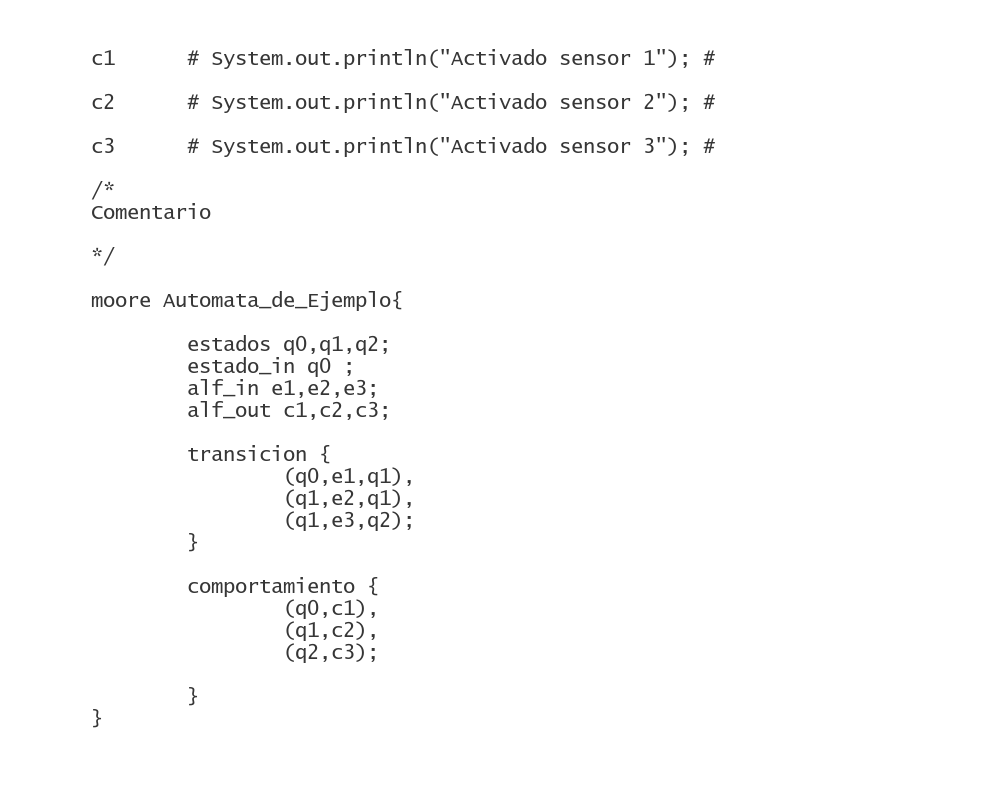
\includegraphics[width=0.8\linewidth]{img/ejemplo}
	\caption{}
	\label{fig:aut}
\end{figure}

	\end{center}
	
	

	\newpage
	\section{EBNF}
			\begin{center}
			\begin{tabular}{lcl}
	

				PROGRAMA & ::= & DEC$\_$COMP AUTOMATA $\{$AUTOMATA$\}$ \\ 
				 
				
				DEC$\_$COMP & ::= &CMP  CODIGO $\{$ CMP CODIGO $\}$ \\ 
			
				CODIGO 	&::= &'$\#$' ASCII '$\#$' \\ 
				
				AUTOMATA & ::= & \textbf{moore} ID CUERPO$\_$AUTOMATA \\
				
			
				CUERPO$\_$AUTOMATA	& ::= & $'\{'$ ESTADOS ESTADO$\_$INI ALF$\_$IN  \\ 
				
					& &  ALF$\_$OUT TRANSICION COMPORTAMIENTOS $'\}'$ \\ 
				
				ESTADOS	& ::= &   \textbf{estados} $\{$ ID ',' $\}$ ID ';'\\ 
				
				 ESTADO$\_$INI &::= & \textbf{estado$\_$in} ID ';'\\ 
				 
				ALF$\_$IN &::= & \textbf{alf$\_$in}  $\{$ EVENTOS ',' $\}$ EVENTOS ';' \\ 
				
				ALF$\_$OUT & ::= &\textbf{alf$\_$out}  $\{$ CMP ',' $\}$ CMP ';'  \\ 
				
				TRANSICION 	 & ::= & \textbf{transicion} $'\{'$ TRANSICION$\_$DEF $\{$ ',' TRANSICION$\_$DEF  $\}$ ';' $'\}'$ \\ 
				
				TRANSICION$\_$DEF & ::= & '(' ID ',' ID ',' ID ')' \\ 
			
				
				COMPORTAMIENTOS	 & ::= &  \textbf{comportamientos} $'\{'$ COMP$\_$DEF $\{$ ',' COMP$\_$DEF $\}$ ';' $'\}'$\\ 
				
				COMP$\_$DEF &  ::= & '(' ID ',' ID ',' ID ')' \\ 
				
				
				CMP  & ::= & 'c'NUMEROS \\ 
				
				NUMEROS &::= & 0 | 1 | .. | 9 \\ 
				
				COMENTARIOS & ::=  & $'/\ast'$ ASCII $'\ast/'$ \\
				
				
			\end{tabular} 	
		\end{center}
	
	
	
	

	\newpage
	\section{Tablas de Tokens}
		
	\begin{center}
		\begin{tabular}{|c|c|c|}
			\hline 
			\textbf{Token} & \textbf{Lexema} & \textbf{Patrón} \\ 
			\hline 
			moore & moore & m$\cdot$o$\cdot$o$\cdot$r$\cdot$e  \\ 
			\hline 
			estados &estados & e$\cdot$s$\cdot$t$\cdot$a$\cdot$d$\cdot$o$\cdot$s \\ 
			\hline 
			estado$\_$in & estado$\_$in & e$\cdot$s$\cdot$t$\cdot$a$\cdot$d$\cdot$o$\cdot$$\_$$\cdot$i$\cdot$n \\ 
			\hline 
			alf$\_$in	& alf$\_$in & a$\cdot$l$\cdot$f$\cdot$$\_$i$\cdot$n \\ 
			\hline 
				alf$\_$out	& alf$\_$out & a$\cdot$l$\cdot$f$\cdot$$\_$o$\cdot$u$\cdot$t \\ 
			\hline 
				transicion	& transicion & t$\cdot$r$\cdot$a$\cdot$n$\cdot$s$\cdot$i$\cdot$c$\cdot$i$\cdot$o$\cdot$n \\ 
			\hline 
				comportamiento	& comportamiento & c$\cdot$o$\cdot$m$\cdot$p$\cdot$o$\cdot$r$\cdot$t$\cdot$a$\cdot$m$\cdot$i$\cdot$e$\cdot$n$\cdot$t$\cdot$o \\ 
			\hline 
			Paréntesis abierto	& ( & ( \\ 
			\hline 
			Paréntesis cerrado	& ) & ) \\ 
			\hline 
			Llave abierta	& $\{$ & $\{$ \\ 
			\hline 
			Llave cerrada	& $\}$ & $\}$ \\ 
			\hline 
			Punto y coma	& ; & ; \\ 
			\hline 
			Coma	& , &  , \\ 
			\hline
			Asterisco barra & $\ast/$  & $\ast$$\cdot/$ \\ 
			\hline 
			Barra asterisco & $/\ast$  &  $/$$\cdot$$\ast$ \\ 
			\hline  
			ID	& hola  & [A-Za-z][A-Zaz0-9$\_$]* \\ 
			\hline 
			CMP	& c1 & c[1-9][0-9]* \\ 
			\hline
		    CODIGO	& $\#$codigo aquí $\#$  & $\#$$\cdot$ codigo aquí $\cdot$$\#$\\ 
			\hline
			
		
	
		\end{tabular} 	
	\end{center}
	\newpage
	\section{¿Cómo se va a construir el procesador del lenguaje diseñado?}
	En el siguiente diagrama tipo T se explica el funcionamiento del procesador que se pretende implementar, tomamos \textbf{ Mor } como lenguaje fuente, y Java como lenguaje objeto, y además el lenguaje que implementa es Java, es decir, nuestro compilador compila a Java, y esta escrito a Java. 
	\newline
	\newline
	Para utilizar ese compilador, utilizamos un compilador auxiliar, que está escrito en código máquina para dar lugar a bytecode, el típico archivo \textbf{.class} que generamos al compilar un \textbf{.java}.
	\newline
	
	Por último tenemos que compilar el bytecode, con un compilador que acepta bytecode escrito en código máquina.
	
	\begin{figure}[h]
		\centering
		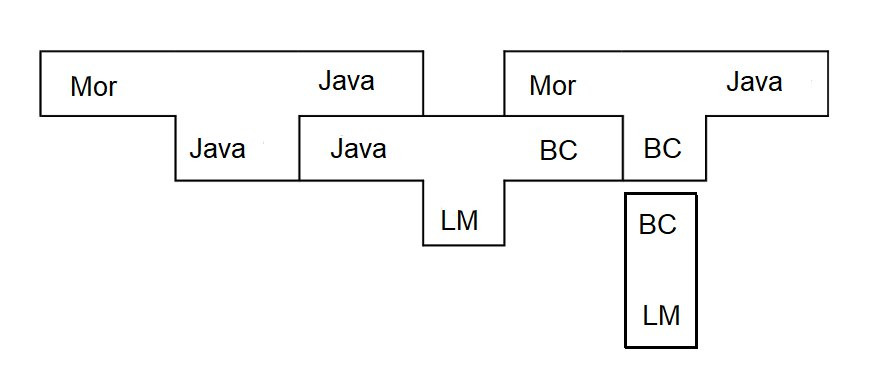
\includegraphics[width=0.7
		\linewidth]{img/photo5978652419892031524}
		\caption{Diagrama tipo T asociado}
		\label{fig:photo5978652419892031524}
	\end{figure}
	
	\newpage
	\begin{thebibliography}{99}
		\bibitem{Moore1} Autómatas de Moore \url{https://es.wikipedia.org/wiki/M%C3%A1quina_de_Moore}
	
	\end{thebibliography}
	
	
	
	
	
\end{document}